%
% File: chap01.tex
% Author: Victor F. Brena-Medina
% Description: Introduction chapter where the biology goes.
%
\let\textcircled=\pgftextcircled
\chapter{Modelling Philosophy and Methods}
\label{chap:intro}

\initial{T}he project was carried out using the 'PyMC3' stack in a Jupyter Notebook editor. A series of strain measurements were simulated and subsequently fit using Least-Squares and Bayesian regression. The measurements were challenging by design, containing noise and outliers, to simulate the results of poor grain-sampling, as described in section x. For clarity, figure 3.1 illustrates the baseline experimental flow for all simulations. \\

As mentioned in section 2.3, the potential for more representative and visualised uncertainties is one of the reasons why Bayesian regression may be useful in stress calculations even if the stress state estimate is of similar accuracy to Least-Squares regression. The feasibility of error estimates yielded by the fits was assessed by comparison with the known true stress tensor from which the strain measurements were generated. The following stress tensor was arbitrarily chosen: 

$$   \sigma_{ij} / MPa  =\begin{bmatrix} \sigma_{11} & \sigma_{12} & \sigma_{13} \\ \sigma_{21} & \sigma_{22} & \sigma_{23} \\ \sigma_{31} & \sigma_{32} & \sigma_{33} \end{bmatrix}   =\begin{bmatrix} 150 & 30 & 0 \\ 30 & 50 & 0 \\ 0 & 0 & 0 \end{bmatrix}$$\\

By treating this stress tensor as belonging to an isotropic ferritic Stainless Steel, the macroscopic Young's Modulus $E$ and Poisson Ratio $\nu$ were taken as: \cite{cambridgeuniversityengineeringdepartment_2003_materials}
$$E = 210000 \ MPa $$
$$\nu = 0.28 $$

\section{Technical Details inc. Code Excerpt}
\label{sec:sec01}

All of the code in this section was adapted from the PyMC3 tutorials and examples \cite{sedar_2010_glm}, and written by or in collaboration with Dr. Matthew Peel, University of Bristol. \\

Although it is not essential to understand the specifics of how this project was implemented in python, the following essential sections of code may be of assistance to individuals wanting to reproduce or verify simulations. For succinctness, some sections such as file management, outlier detection and the prior effects simulation have been omitted; The complete Jupyter Notebooks are available upon request. \\

The following modules were installed and imported for use:

 \begin{figure}[H]
 	\centering
 	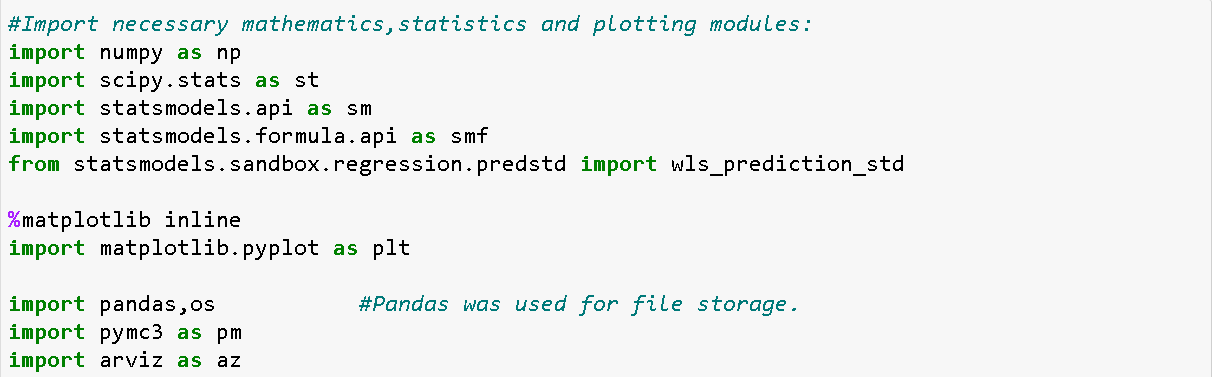
\includegraphics[width=0.8\linewidth]{chapters/chapter02/fig02/imports.png}
 %	\mycaption[figurex]{Developmental zones of an Arabidopsis root. Figure reproduced from \cite{griersonRH}.}
 %	\label{fig:RHP02}
 \end{figure}

Recalling from section 2.1 that the relationship between strain in a given location, stress tensor components and detector angle, $\gamma$, can be described by equation 2.x and that $h_{ij}$ can be simplified to be a function of only $\gamma$ for high energy X-Ray diffraction (low $\theta$) \cite{he_2018_twodimensional} $h_{ij}$ and $p_{ij}$ were calculated for incremented $\gamma$.

 \begin{figure}[H]
 	\centering
 	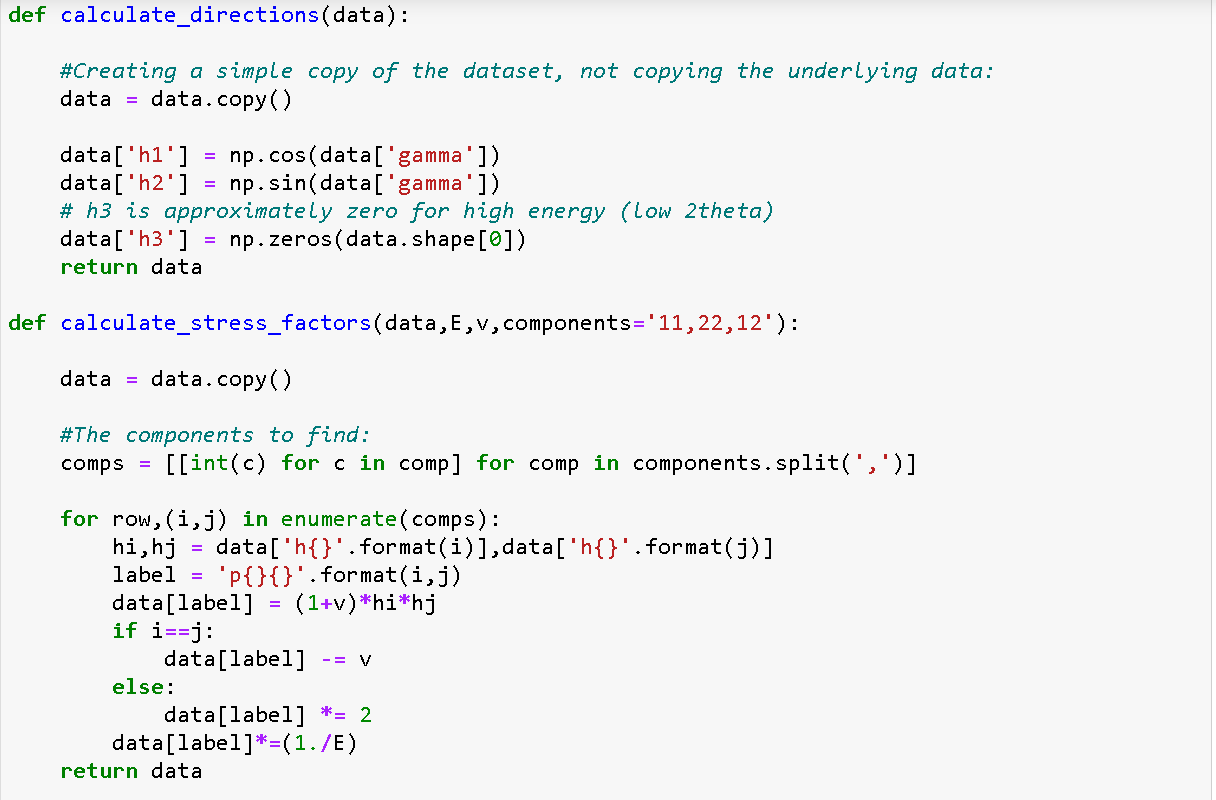
\includegraphics[width=0.8\linewidth]{chapters/chapter02/fig02/findhp.png}
 %	\mycaption[figurex]{Developmental zones of an Arabidopsis root. Figure reproduced from \cite{griersonRH}.}
 %	\label{fig:RHP02}
 \end{figure}

A strain distribution was generated at each location and statistical noise, the origin and nature of which was discussed in section 2.2, was added to create simulated strain 'measurements'.

 \begin{figure}[H]
 	\centering
 	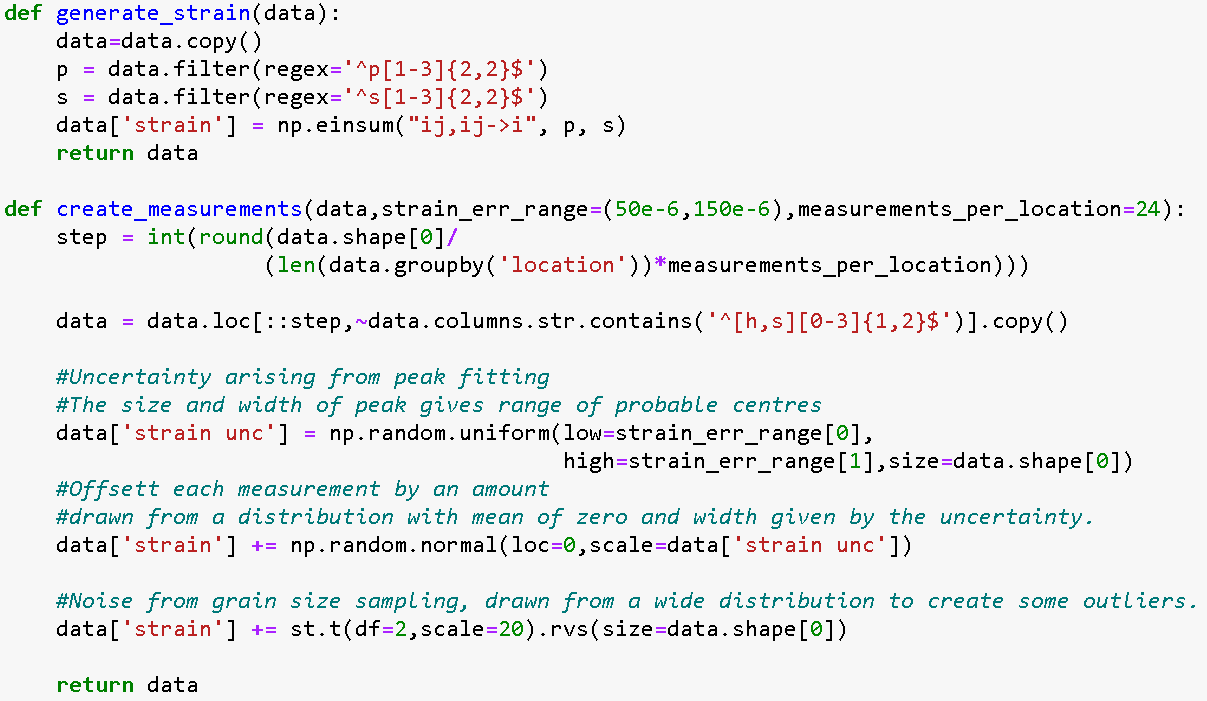
\includegraphics[width=0.8\linewidth]{chapters/chapter02/fig02/generatemeasurements.png}
 %	\mycaption[figurex]{Developmental zones of an Arabidopsis root. Figure reproduced from \cite{griersonRH}.}
 %	\label{fig:RHP02}
 \end{figure}

Weighed Least-Squares regression was used to fit the simulated strain measurements, in order to solve for stress tensor components.



 \begin{figure}[H]
 	\centering
 	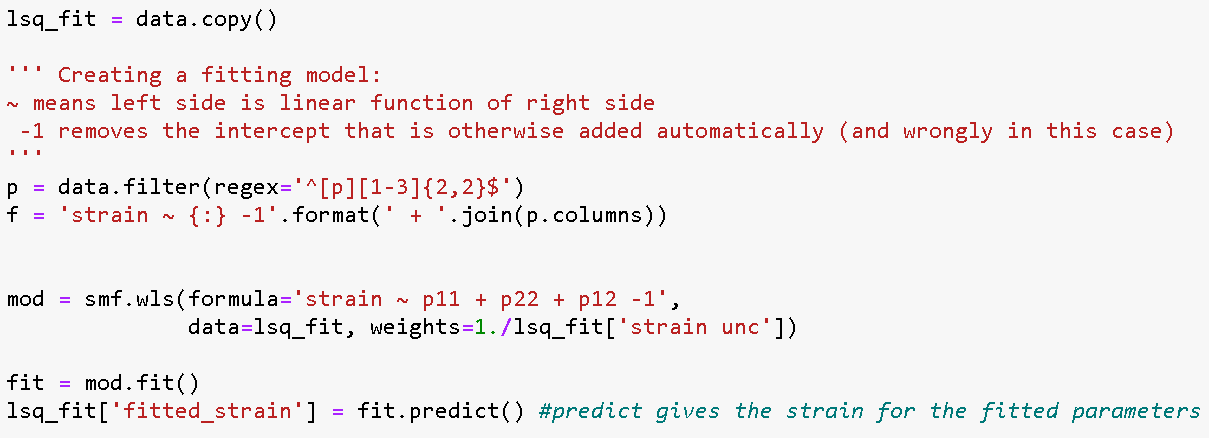
\includegraphics[width=0.8\linewidth]{chapters/chapter02/fig02/LSQ.png}
 %	\mycaption[figurex]{Developmental zones of an Arabidopsis root. Figure reproduced from \cite{griersonRH}.}
 %	\label{fig:RHP02}
 \end{figure}

Bayesian regression was used to fit the same strain measurements. The key differences in implementation, aside from the increased computational demands and length of code, are the incorporation of prior knowledge about the numerical value of the data, as well as the option to specify the shape of the likelihood function. 

 \begin{figure}[H]
 	\centering
 	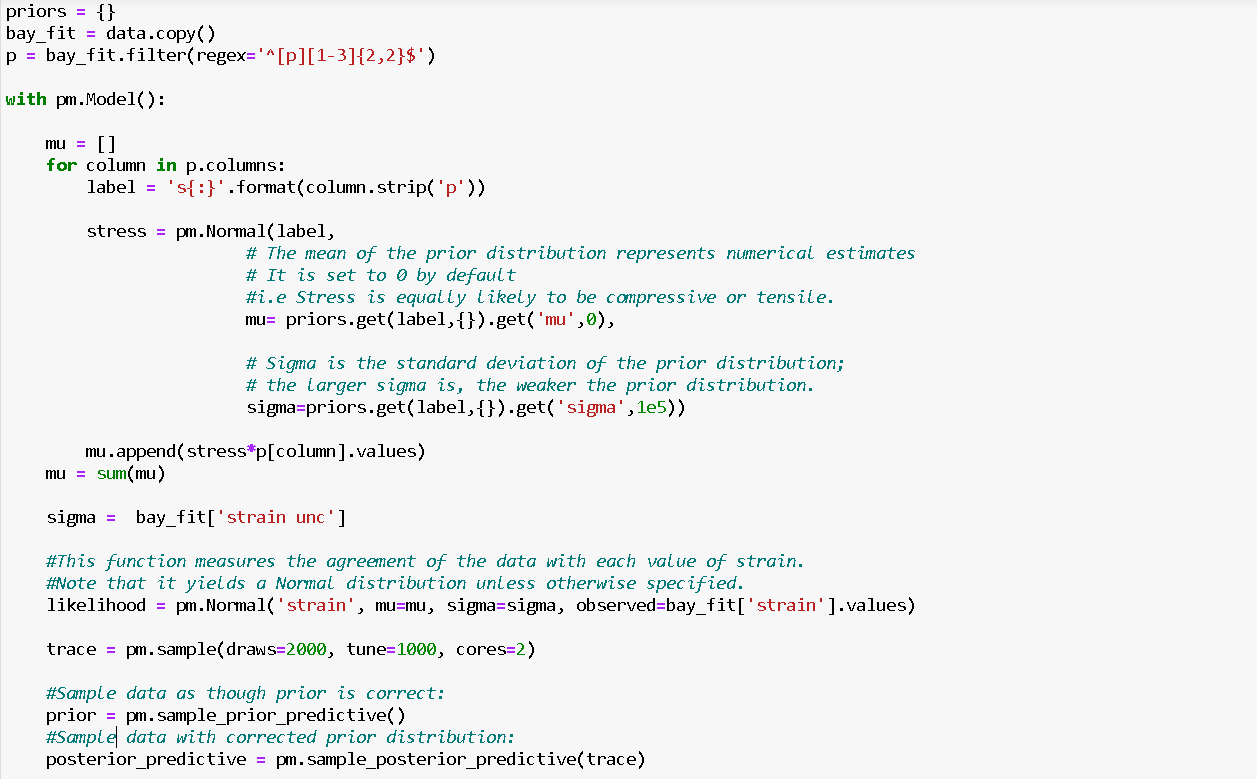
\includegraphics[width=0.8\linewidth]{chapters/chapter02/fig02/bayesfit.png}
 %	\mycaption[figurex]{Developmental zones of an Arabidopsis root. Figure reproduced from \cite{griersonRH}.}
 %	\label{fig:RHP02}
 \end{figure}

\newpage
\section{Outline of Simulations}
\label{sec:sec01}

\subsection{The Extent of the Prior Distribution's Influence on Fit Outcome}
\label{subsec:subsec01}

The influence of prior knowledge on the fit outcome of Bayesian regression has been a subject of debate \cite{andrew_2015_can}, which highlights the importance of answering the question: "To what extent does the fit outcome validate the prior distribution?"\\

    It has been argued that the ability to inform the fit outcome using data collected elsewhere, such as hole drilling or other stress analysis techniques, is valuable and can make the fit more realistic.\cite{shaver_2017_a} Conversely, incorporating prior or assumed knowledge about a data-set into the fitting model could introduce a level of subjectivity to the fit outcome, potentially reducing the validity of the result, especially if the assumptions are inaccurate \cite{andrew_2015_can}. Supporters of Bayesian regression have argued that the choice of prior is irrelevant if the data-set is large enough, citing Bernstein–Von Mises' theorem \cite{Giordano_Kekkonen_2018}, which implies that the posterior distribution converges to the result implied by the data, i.e that Bayesian regression favours the data over the prior.\\ 

The impact of the prior distribution on the Bayesian fit outcome was tested in the context of stress analysis by simulating two sets of strain measurements, one with high noise and one with low noise. Each set of measurements was fit using Bayesian regression with increasing prior strength. To assess the impact of a potentially incorrect prior, the simulation was repeated for 3 numerical values of the prior distribution's mean, which represents the mean stress: 0, 150 (which was the true stress) and 300 MPa. The result, which is that changes to the mean of the prior distribution have a marginal impact on fit outcome, is detailed in section 4.1.1\\

Furthermore, the impact of changes to the nature of the Bayesian likelihood function were also tested by comparing Least-Squares regression with simple Bayesian regression, wherein the likelihood function \cite{dendukuri_2018_lecture} is normally distributed, and robust Bayesian, where the likelihood function was T-distributed.A T distributed likelihood function potentially allows better handling of extreme outliers which can arise from grain sampling statistics.\cite{lange_1989_robust}\\

 \begin{figure}[H]
 	\centering
 	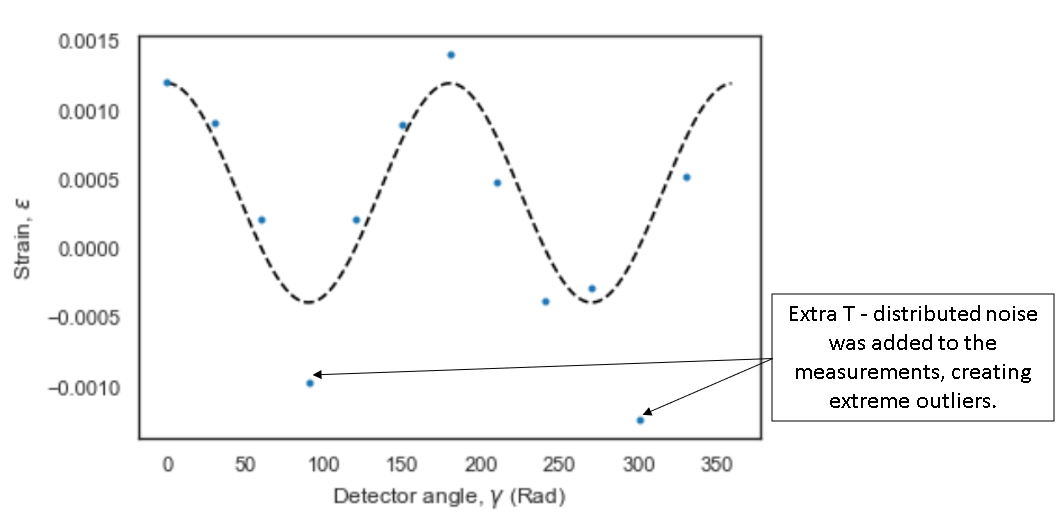
\includegraphics[width=0.8\textwidth]{chapters/chapter02/fig02/outliers.png}
 	\mycaption
 	{Strain measurements simulated using a known stress tensor. The measurements contain Normally distributed noise to simulate diffraction uncertainty in diffraction peak position, and extra Student's T-distributed noise to simulate poor grain-sampling statistics.}
    \label{fig:RHP02}
 \end{figure}
 
Fit comparisons were carried out on samples with manually introduced extreme outliers, such as that plotted in figure 3.1. The results, detailed in section 4.1.2, imply that simple Bayesian yields almost identical fit outcomes to Least-Squares regression; Furthermore, that robust Bayesian regression can yield more accurate fit outcomes with more realistic confidence intervals than both simple Bayesian and Least-Squares regression for samples with extreme outliers.\\


\subsection{Comparing Weighed Least-Squares to Robust Bayesian Regression}
\label{subsec:subsubsec01}

In this section, the methodology and reasoning behind some of the simulations tested is outlined. Although more measurements were simulated and fit using linear regression, the ones which best illustrate findings were chosen for conciseness. For the method by which these samples were generated and fit, please refer back to section 3.1.\\

\subsubsection{Simulated Measurements with Normally Distributed Errors}
%\label{subsubsec:subsubsec01}

The simplest origin of errors in X-Ray diffraction strain measurements is the uncertainty associated with diffraction peak position. This uncertainty can easily be resolved via peak width analysis, and is often known when fitting the strain measurements.\\

The first two examples of simulated strain measurements contain only Normally distributed noise to simulate the uncertainty associated with peak location. One sample (fig. 3.2) simulates a setup analogous to higher penetration neutron diffraction, which is less sensitive to surface stress and therefore has low uncertainty; The other (fig. 3.3) contains measurements with high noise, to simulate a setup analogous to in-lab X-Ray diffraction, which has lower penetration and is therefore more sensitive to surface stress differences. The two samples were fit using Weighed Least Squares and Robust Bayesian regression. The results, which imply that Bayesian regression does not yield a significantly higher quality fit for measurements with Normally distributed errors, are detailed in section 4.2. 


 \begin{figure}[h]
 	\centering
 	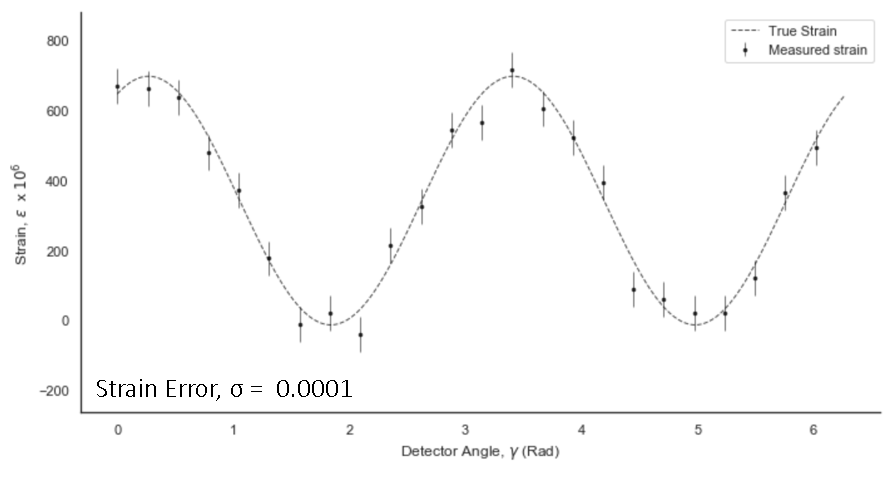
\includegraphics[width=0.8\textwidth]{chapters/chapter02/fig02/sample1.png}
 	\mycaption
 	{Simulated strain measurements with low, Normally distributed noise, mimicking deep penetration (e.g Neutron) diffraction measurements of a material with a uniform grain structure. Standard deviation of error distribution, $\sigma$ = 0.0001.}
    \label{fig:RHP02}
 \end{figure}

 
  \begin{figure}[H]
 	\centering
 	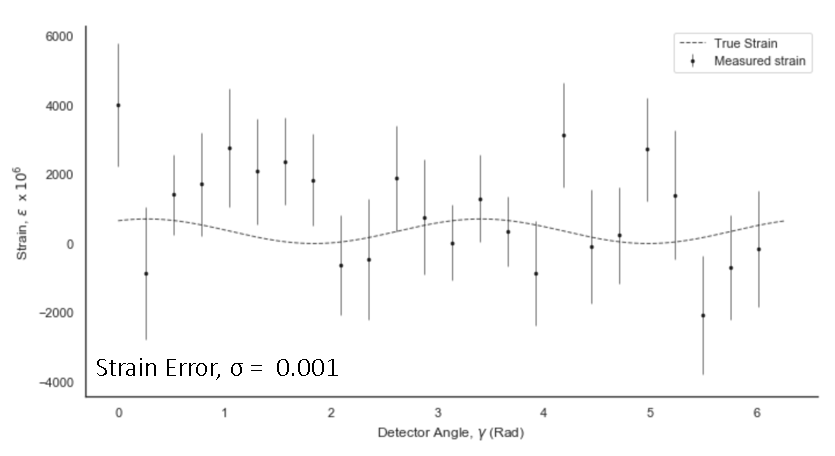
\includegraphics[width=0.8\textwidth]{chapters/chapter02/fig02/sample6.png}
 	\mycaption
 	{Simulated strain measurements with high, Normally distributed noise, mimicking low penetration (e.g laboratory X-Ray) diffraction measurements of a material with a uniform grain structure. Standard deviation of error distribution, $\sigma$ = 0.001.}
    \label{fig:RHP02}
 \end{figure}

\subsubsection{Simulated Measurements with T- Distributed Errors}
%\label{subsubsec:subsubsec01}

The following two examples of simulated strain measurements contain only Student's T distributed noise to simulate the uncertainty associated with grain sampling statistics; This distribution allows for the creation of outliers, as it has wide tails. These samples were fit using Weighed Least Squares and Robust Bayesian, with the results detailed in section 4.3.

  \begin{figure}[H]
 	\centering
 	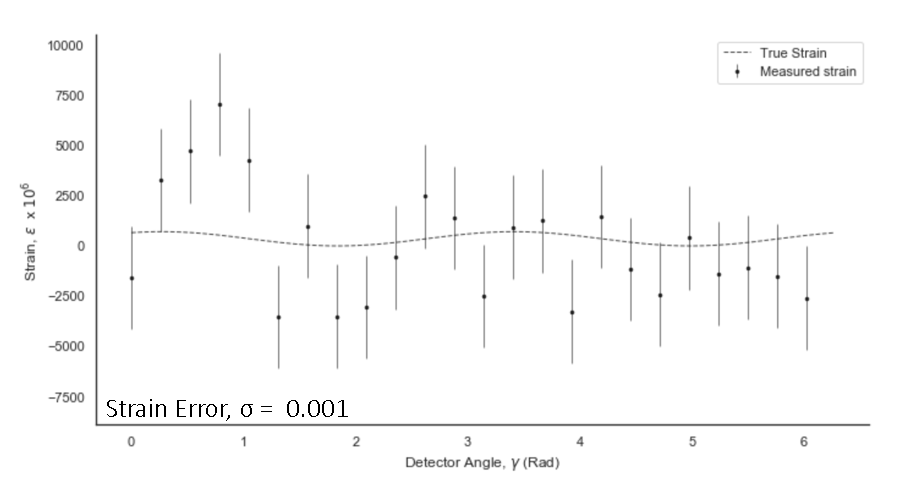
\includegraphics[width=0.8\textwidth]{chapters/chapter02/fig02/sample3.png}
 	\mycaption
 	{Simulated strain measurements with high, T - distributed noise, to simulate the uncertainty from grain sampling statistics in a sample with non-uniform grain sizes. Standard deviation of error distribution, $\sigma$ = 0.001; Degrees of freedom of T distribution = 3 (100 = Normal distribution).}
    \label{fig:RHP02}
 \end{figure}

\subsubsection{Samples with Manually Introduced Outliers}
%\label{subsec:subsec01}

Recalling from section 2.2 that real X-Ray diffraction strain measurements contain both uncertainties associated with peak position and with grain sampling statistics. The following samples were created with a combination of Normally distributed noise and T-distributed noise, with two degrees of freedom, simulating peak position and grain sampling uncertainties respectively.\\

The same samples were used later to test automated anomaly detection, the results for which are detailed in section 4.5.


  \begin{figure}[H]
 	\centering
 	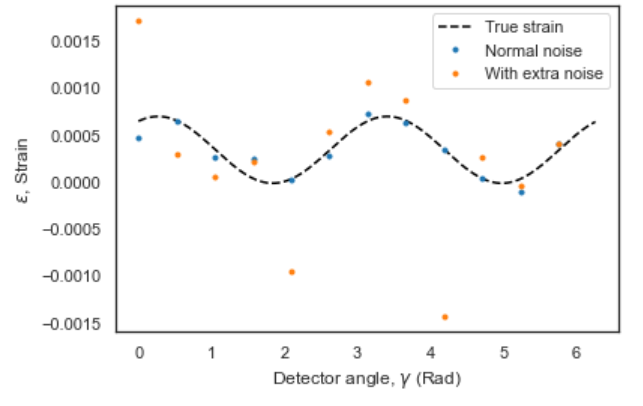
\includegraphics[width=0.8\textwidth]{chapters/chapter02/fig02/sample9.png}
 	\mycaption
 	{Simulated strain measurements with a combination of Normally and T - distributed noise, to simulate both grain sampling and peak position uncertainties. Standard deviation of Normal error distribution, $\sigma$ = 0.0001; Degrees of freedom of T distribution = 2 (100 = Normal distribution).}
    \label{fig:RHP02}
 \end{figure}
 
   \begin{figure}[H]
 	\centering
 	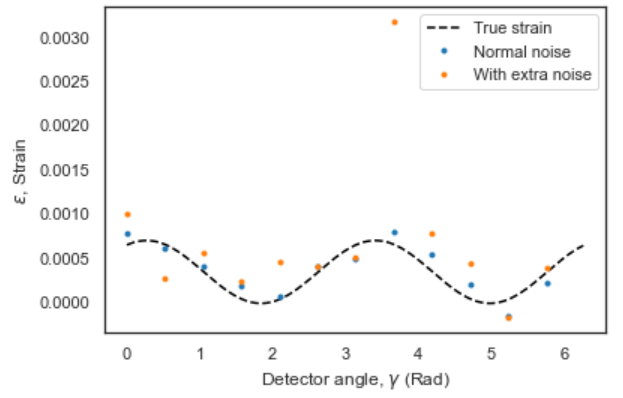
\includegraphics[width=0.8\textwidth]{chapters/chapter02/fig02/s10.png}
 	\mycaption
 	{Simulated strain measurements with a combination of Normally and T - distributed noise, to simulate both grain sampling and peak position uncertainties. Standard deviation of Normal error distribution, $\sigma$ = 0.00005; Degrees of freedom of T distribution = 2 (100 = Normal distribution).}
    \label{fig:RHP02}
 \end{figure}

\subsection{Outlier Detection Using Bayesian}
\label{subsec:subsec01}

As discussed in section 2.2, Least-Squares regression is known to be poor at handling outliers unless data is manually optimised, a process which can be tedious and subjective. As a result, fit outcomes could be heavily skewed by as few as one extreme anomaly, perhaps resulting from an abnormally large grain. From the simulation described section 3.2.1 and its results in section 4.1, it was seen that changes to the likelihood function of Bayesian regression can yield a significantly different, and sometimes more accurate, fit outcome. Previously, the likelihood function was changed to a Student's T distribution, although in theory any Gaussian-like distribution can be used. \\

The aim of this simulation was to assess the impact of changing the likelihood function to a Bernoulli distribution and use it to assign measurements as inliers or outliers and weigh them accordingly, essentially automating the anomaly detection process. The cut-off point for a measurement to be labelled an outlier was for the algorithm to assign it as such 80\% or more of the time. The 80\% cut-off is arbitrary, and thus subjective, yet remains more objective than manual outlier detection, as the criterion for a measurement to be labelled an anomaly is the same for all measurements.\\

The results, detailed in section 4.5, were that the outlier detection was successful for extreme outliers and the resulting fit was of similar quality to robust (T - distributed likelihood) Bayesian regression, and was more accurate in some cases. Importantly, the algorithm did not incorrectly label any inliers as outliers.

% %A figures matrix.
% \begin{figure}[t!]
% \centering
% \begin{minipage}{3.3cm}
%     \centering
%     \subtop[]{\includegraphics[height=0.28\textheight]{fig01/Nswellings}\label{sf:multiRH02a}}
% \end{minipage}
% \hspace{0.5cm}
% \begin{minipage}{3.3cm}
%     \centering
%     \subtop[]{\includegraphics[height=0.27\textheight]{fig01/Mswellings}\label{sf:multiRH02b}}
% \end{minipage}
% \hspace{1.3cm}
% \begin{minipage}{3.3cm}
%     \centering
%     \subtop[]{\includegraphics[height=0.27\textheight]{fig01/rhd1}\label{sf:multiRH02c}}
% \end{minipage}
% \\ \vspace{0.1cm}
% \begin{minipage}{10cm}
%     \centering
%     \subtop[]{\includegraphics[height=0.145\textheight]{fig01/mutantrhd6}\label{sf:multiRH02d}}
% \end{minipage}
% \\ \vspace{0.1cm}
% \begin{minipage}{10cm}
%     \centering
%     \subtop[]{\includegraphics[height=0.16\textheight]{fig01/auxab}\label{sf:multiRH02e}}
% \end{minipage}
% \mycaption[Hair-forming mutant cells.]{(a) A mutant RH cell. Asterisks show multiple sites of RH initiation in a single root hair cell (indicated by the arrows). Figure reproduced from \cite{rigas01}. (b)~Hair-forming cell with three RH initiation locations. The bar represents $50\mu m$. Figure reproduced from \cite{massuci01}. (c) Large bump in mutant {\itshape rhd1}. Figure reproduced from \cite{griersonRH}. (d) Mutant overexpressing gene {\itshape ROP2}; from right-hand to left-hand, numbers indicate progressive snapshots at different times. RH initiation sites are indicated by the arrows. The bar represents $75\mu m$. Figure reproduced from~\cite{mjones01}. (e)~Mutants affected by auxin. On the left-hand side, RH site is farther away from the apical end (left arrow cap); on the right-hand side, multiple RH locations (arrows). Figure reproduced from~\cite{payne01}.}



%=========================================================g